Validation selects Fine HOG + RBF SVM. On the official test set, it achieves 90.87\% accuracy and macro F1 0.9084. Among the eight core models, validation selects Pixels + RF, whose test accuracy is 87.61\%. We fixed both choices before examining this experiment's test scores.
\begin{table}[t]\centering\caption{Test results using 48,000 training images. An asterisk marks an additional RBF experiment.}\label{tab:results}
\small\begin{tabular}{lrr}\toprule Model & Accuracy (\%) & Macro F1 \\ \midrule
Fine HOG + RBF SVM* & 90.87 & 0.9084 \\
Pixels + RBF SVM* & 89.73 & 0.8971 \\
Pixels + RF & 87.61 & 0.8747 \\
HOG + RBF SVM* & 87.70 & 0.8769 \\
Pixels + k-NN & 85.09 & 0.8515 \\
Pixels + LR & 83.96 & 0.8390 \\
Pixels + linear SVM & 83.97 & 0.8373 \\
HOG + LR & 84.55 & 0.8450 \\
HOG + linear SVM & 84.01 & 0.8385 \\
HOG + RF & 84.59 & 0.8455 \\
HOG + k-NN & 83.81 & 0.8382 \\
\bottomrule\end{tabular}\end{table}
\begin{figure}[t]\centering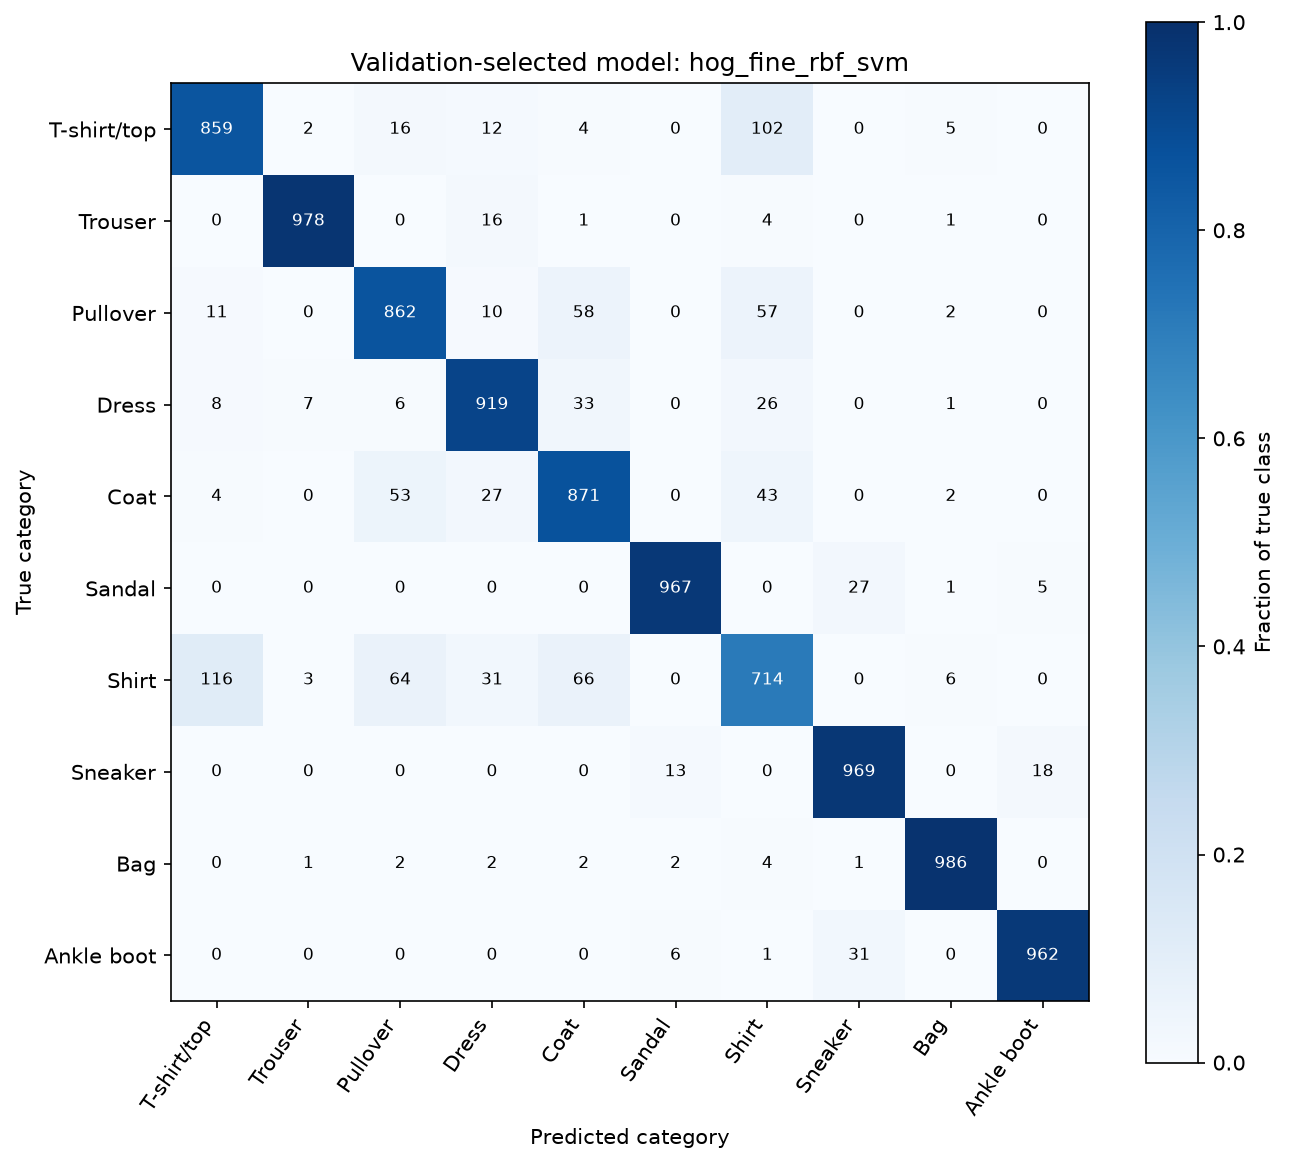
\includegraphics[width=\columnwidth]{selected_confusion.png}\caption{Official test confusion matrix for the selected model. Cells show counts, with shading normalized within each true class.}\end{figure}
\begin{table}[t]\centering\caption{Recall by category for the model selected on validation data.}\begin{tabular}{lr}\toprule Category & Recall (\%) \\ \midrule
T-shirt/top & 85.9 \\
Trouser & 97.8 \\
Pullover & 86.2 \\
Dress & 91.9 \\
Coat & 87.1 \\
Sandal & 96.7 \\
Shirt & 71.4 \\
Sneaker & 96.9 \\
Bag & 98.6 \\
Ankle boot & 96.2 \\
\bottomrule\end{tabular}\end{table}
The most frequent upper-body mistakes are Shirt to T-shirt/top: 116; T-shirt/top to Shirt: 102; Shirt to Coat: 66. Similar shapes and textures at this resolution may contribute to these errors, though we have not established the cause. The notebook includes upper-body examples sampled with a fixed seed.
The selected model uses 17,835 support vectors and 52.74 MiB of serialized storage. Median single-image latency is 10.169 ms, with p95 15.732 ms. Batch throughput is 59.5 images/s under the common protocol. These timings exclude file decoding and model loading.
